\documentclass[11pt]{beamer}
\usepackage[utf8]{inputenc}
\usepackage[T1]{fontenc}
\usepackage{lmodern}
\usepackage[english,spanish]{babel}
\usetheme{CambridgeUS}
\usepackage{graphicx}
\begin{document}
    \author{Dr. Alejandro Rodr\'iguez}
    \title{Estadística Inferencial}
    %\subtitle{}
    %\logo{}
    %\institute{}
    %\date{}
    %\subject{}
    %\setbeamercovered{transparent}
    %\setbeamertemplate{navigation symbols}{}
    \begin{frame}[plain]
        \maketitle
    \end{frame}

    \section{Introducción a la estadística inferencial.}
      \begin{frame}{Estadística inferencial}
        \begin{block}{Estadística inferencial}
            Se llama estadística inferencial o inferencia estadística a la rama de la Estadística encargada de hacer \textbf{deducciones}, es decir, \textbf{inferir propiedades}, \textbf{conclusiones} y \textbf{tendencias}, a partir de una muestra del conjunto. \textbf{Su papel es interpretar, hacer proyecciones y comparaciones.}
        \end{block}
      \end{frame}


      \begin{frame}{Estadística inferencial}
          \begin{block}{Estadística inferencial}
              \begin{itemize}
                  \item Estimación estadística
                  \item Prueba de Hipótesis
                  \item Regresión Lineal y Correlación
                  \item Diseño de experimentos
              \end{itemize}
          \end{block}
      \end{frame}

      \subsection{Estimación estadística}
        \begin{frame}{Estimación estadística}
            \begin{block}{Estimación estadística}
                La estimación es la determinación de un elemento o factor. Esto, usualmente tomando como referencia una base o conjunto de datos.
            \end{block}
            \pause
            La estimación es un cálculo que se realiza a partir de la evaluación estadística. Dicho estudio suele efectuarse sobre una muestra y no sobre toda la población objetivo.
            Sea $X_1, X_2, X_3, \ldots , X_n $ una muestra aleatoria de una distribución, un estimador es un estadístico $\hat{\theta}=T(X_1, X_2, X_3, \ldots , X_n)$ que sirve para estimar el valor $\theta$.

            \pause
            Nos sirve para calcular indicadores estadísticos como la \textbf{media}, la\textbf{ mediana}, \textbf{moda} y \textbf{desviación estándar}.
        \end{frame}

        \begin{frame}{Estimación estadística. Puntual}
            \begin{block}{Estimación estadística Puntual}
                La estimación puntual consiste en encontrar un valor para $\theta$, denotado por  $\hat {\theta }$. Es decir seleccionar aquel estadístico que mejor nos permita describir la muestra.

                \pause
                \textbf{Ejemplo:} Por ejemplo, si se pretende estimar la talla media de un determinado grupo de individuos, puede extraerse una muestra y ofrecer como estimación puntual la talla media de los individuos.
            \end{block}

        \end{frame}

        \begin{frame}{Estimación estadística. Puntual}
          Podría ser que ni el estimador eficaz estime con exactitud el parámetro de la población. Sabiendo que la exactitud de la estimación aumenta cuando las muestras son grandes; pero incluso así no tenemos razones para esperar que una estimación puntual de una muestra dada sea exactamente igual al parámetro de la población que se
supone debe estimar.

          \vspace{15px}
          Hay muchas situaciones en que es preferible determinar un intervalo dentro del cual esperaríamos encontrar el valor del parámetro. Tal intervalo se conoce como \textbf{estimación por intervalo}.
        \end{frame}
        \begin{frame}{Estimación estadística. Estimación por intervalo}
           En la estimación por intervalo calculamos el intervalo de confianza. Este intervalo intervalo $E_{+}< \bar {x} < E_{-}$ , que se calcula a partir de la muestra seleccionada, se llama entonces intervalo de confianza y los extremos, $E_{+}$ y $E_{-}$, se denominan límites de confianza inferior y superior.

          \begin{figure}
              \centering
              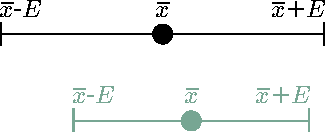
\includegraphics[width=0.5\linewidth]{images/inferencial1}
              \caption{Ejemplo de dos posibles valores y sus intervalos de confianza.}
              \label{fig:inferencial1}
          \end{figure}
        \end{frame}

        \begin{frame}{Estimación estadística. Estimación por intervalo}
            \begin{figure}
                \centering
                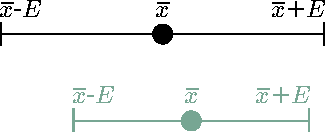
\includegraphics[width=0.5\linewidth]{images/inferencial1}
                \caption{Ejemplo de dos posibles valores y sus intervalos de confianza.}
                \label{fig:inferencial11}
            \end{figure}
            Para hacer la estimación de los límites de confianza emplearemos la siguiente expresión:
            $$E_{\pm}=\dfrac{1.96 \times \sigma}{\sqrt{n}} $$
            Siendo: $\sigma$ desviación estándar $\sigma=\sqrt{\dfrac{\sum _{i=1}^{n}(x_i- \bar{x})^2}{n-1}}$ y $n$ el numero de elementos.
        \end{frame}

     \subsection{Prueba de significación o Hipótesis}
       \begin{frame}{}
         \begin{center}
             \textbf{\huge Prueba de significación o Hipótesis}
         \end{center}
       \end{frame}
       \begin{frame}{Prueba de Hipótesis}
         La \textbf{verificación de hipótesis}  es el proceso que lleva a juzgar la credibilidad de declaraciones tentativas (hipótesis) relativas a las poblaciones de las que fueron extraídas las muestras.

         \begin{block}{Ejemplo}
             Analizamos el contenido de sodio en unas muestras de un lote de unas galletas y obtenemos un valor medio de $352 mg$. Afirmamos entonces que el contenido medio de sodio en ese lote es de $352 mg$.

             \pause
             Entonces otra persona, que puede ser, nuestro cliente, obtiene de unas muestras de ese mismo lote un valor medio del contenido de sodio igual a $375 mg$.

             \pause
             ¿Contradice este resultado o no mi afirmación de que el contenido medio es de 352 mg? ¿Aceptará o rechazará el lote mi cliente?
         \end{block}
         \pause
         Para esclarecer esto tenemos que seguir los procedimientos de las pruebas de hipótesis.
    \end{frame}

       \begin{frame}{Prueba de Hipótesis}
         \pause
         Lo que se puede hacer es afirmar que tiene tal o cual probabilidad  de ser verdadera o falsa. Si la probabilidad de ser verdadera es muy alta (95\% o 99\%) por ejemplo, se concluye que la hipótesis es altamente creíble y se califica provisionalmente como cierta.

         Si no se consigue probar que es verdadera (se rechaza), se acepta provisionalmente como falsa.

       \end{frame}

       \begin{frame}{Prueba de Hipótesis}
         Casi siempre se plantean dos hipótesis: \textbf{la hipótesis nula} y \textbf{su contraria, la hipótesis alternativa}, planteándose generalmente como: $H_0$ y $H_1$.


         Pasos a seguir para la prueba de hipótesis:
         \begin{itemize}
            \item Definir la hipótesis a contrastar.
            \item Definir la prueba estadística a emplear.
            \item Establecer el nivel de significación.
            \item Hacer la experimentación (muestrear y evaluar el o los estadísticos.
            \item Tomar la decisión sobre la hipótesis.
         \end{itemize}
       \end{frame}

       \subsubsection*{Distribuciones F-Fisher}
         \begin{frame}
           \textbf{\begin{center}
                 \huge Prueba de Hipótesis  F-Fisher
           \end{center}}
         \end{frame}


         \begin{frame}{Distribuciones F-Fisher}
           Prueba $F$ para igualdad de varianzas

           Hipótesis nula: $H_0: \sigma^2_1 = \sigma^2_2$

           Valor estadístico de prueba: $f = s^2_1/s^2_2$
           Siendo $\alpha$ el grado insignificancia, por lo tanto $1 -\alpha$ cuantificaría el nivel de confianza.

           \vspace{1px}
           \begin{center}
             \begin{tabular}{cc}
                 Hipótesis alternativa          &   Región de rechazo para una prueba de nivel $\alpha$\\
                 $H_a: \sigma^2_1 > \sigma^2_2$ & $f \geq F_{\alpha,m-1,n-1}$ \\
                 $H_a: \sigma^2_1 < \sigma^2_2$ & $f \leq F_{1-\alpha,m-1,n-1}$ \\
                 $H_a: \sigma^2_1 \neq \sigma^2_2$ & o $f \geq F_{\alpha/2,m-1,n-1}$ o $f \leq F_{1-\alpha/2,m-1,n-1}$ \\
             \end{tabular}
           \end{center}

           \vspace{1px}

           Como los valores críticos se tabulan sólo para $\alpha$ = 0.10, 0.05, 0.01 y 0.001. Con software estadístico se obtienen otros valores críticos $F$.
       \end{frame}

         \begin{frame}{Distribuciones F-Fisher. Ejemplo}
           \begin{block}{Ejemplo}
             La variabilidad en la cantidad de grasa presente en un lote de un complemento dietético, utilizada para un proceso de fabricación de un alimento, depende del origen del complemento. Un fabricante que recibe el complemento de dos proveedores \textbf{1} y \textbf{2}, hizo una comparación analizando muestras de ambos proveedores. Muestras de $n_1=10$ y $n_2=16$ mediciones de dos lotes produjeron las varianzas:

             $S^2_1=1.25$ y $S^2_2=0.5$

             ¿Presentan los datos evidencia suficiente para indicar que la variabilidad en el contenido de grasa es menor para el producto que se recibe del proveedor 2? Realice una prueba con un a o $\alpha$ = 0.05.
         \end{block}
        \end{frame}
         \begin{frame}{Distribuciones F-Fisher. Ejemplo}
           \begin{block}{Soluci\'on}
             Tenemos nuestras hipótesis nula, la cual aceptamos a priori:

             $H_a: \sigma^2_1 > \sigma^2_2\quad : \quad f \geq F_{\alpha,m-1,n-1}$

             Y rechazamos si:

             $f \geq F_{\alpha,m-1,n-1}$

             Luego, debemos buscar en tablas con una exactitud de 0.05 el valor de $F_{tabla}$.
             \pause
             $f \geq 2.5876$

             $f_{calculado} = \dfrac{1.25}{0.5}=2.5$
             \pause
             \vspace{0.2px}

             Como 2.5 $<$ 2.5876 no se rechaza $H_0$, y se concluye con un $\alpha= 0.05$ que no existe suficiente evidencia para decir que la variabilidad del contenido de grasa del complemento del proveedor 2 es menor que la del complemento suministrado por el proveedor 1.
           \end{block}
        \end{frame}

         \begin{frame}{Distribuciones F-Fisher. La Tabla}
           \begin{figure}
             \centering
             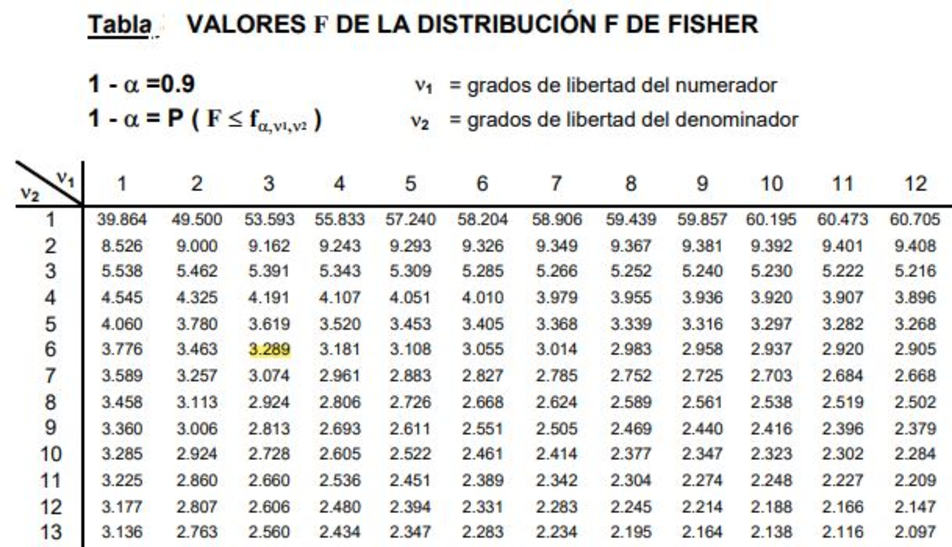
\includegraphics[width=0.7\linewidth]{images/estadistica14}
             \label{fig:estadistica14}
           \end{figure}
           La columna indica el grado de libertad del numerador y la fila el grado de libertad del denominador.
           La Figura\ref{fig:estadistica14} muestra una sección de la tabla de la distribución F para el caso de un nivel de significancia de 10\%, es decir $\alpha = 0.1$. Aparece resaltado el valor de \textbf{F} cuando $\nu_1= 3$ y $\nu_2 = 6$ con nivel de confianza $1-\alpha  = 0.9$ es decir 90\%.
         \end{frame}

     \subsection{Regresión lineal simple y correlación}
       \begin{frame}{}
           \begin{center}
               \textbf{\huge Regresión lineal simple y correlación}
           \end{center}
       \end{frame}

       \begin{frame}{Regresión lineal simple}
           \begin{block}{}
               En la práctica a menudo se requiere resolver problemas que implican conjuntos de variables de las cuales se sabe que tienen alguna relación inherente entre sí.
           \end{block}
           \pause
           Sin embargo:
           \begin{block}{}
             \begin{itemize}
                 \item No todas las casas ubicadas en la misma zona del país, con la misma superficie de construcción, se venden al mismo precio.
                 \item Varios automóviles con un motor del mismo volumen; no tienen que tener el mismo rendimiento de combustible
             \end{itemize}
           \end{block}
       \end{frame}
       \begin{frame}{Regresión lineal simple}
           \begin{block}{}
              Una forma razonable de relación entre la respuesta $Y$ y
el \textbf{regresor} $x$ es la relación lineal.

              $$ Y = \beta_0+\beta_1x$$

              en la que $\beta_0$ es la intersección y $\beta_1$ es la pendiente.
           \end{block}
           \pause
           \begin{block}{Análisis de regresión}
               El
concepto de \textbf{análisis de regresión} se refiere a encontrar la mejor relación entre $Y$ y $x$ cuantificando la fuerza de esa relación, y empleando métodos que permitan predecir los
valores de la respuesta dados los valores del regresor $x$.
           \end{block}
       \end{frame}

       \begin{frame}{correlación}
           \textbf{\begin{center}
                  \huge Correlación
           \end{center}}
       \end{frame}

       \begin{frame}{Correlación}
         Tomemos a $X$ como la antigüedad de un automóvil usado y $Y$ representa su
precio, se esperaría que los valores grandes de $X$ correspondan a
valores pequeños de $Y$ y que los valores pequeños de $X$ correspondan a valores grandes
de $Y$.
         \pause
         \begin{block}{Correlación}
           El \textbf{análisis de correlación} intenta medir la fuerza de tales relaciones entre dos variables por medio de un solo número denominado \textbf{coeficiente de correlación}.
         \end{block}
         \pause
         $r_{xy}$ representa el coeficiente de correlación de Pearson.
         $$ r_{xy}=\dfrac{\sum _{i=1}^{n}(x_i-\bar {x})(y_i-\bar {y})}{\sqrt{\sum _{i=1}^{n}(x_i-\bar {x})^2\sum _{i=1}^{n}(y_i-\bar {y})^2}}  $$

        \end{frame}

        \begin{frame}{Correlación. Interpretación}

            El valor del índice de correlación varía en el intervalo $[-1,1]$, indicando el signo el sentido de la relación:
            \begin{itemize}
                \item Si $r=1$, existe una \textbf{correlación positiva perfecta}. El índice indica una \textbf{dependencia total} entre las dos variables denominada relación directa: \textit{cuando una de ellas aumenta, la otra también lo hace en proporción constante}.
                \pause
                \item Si $0<r<1$ entonces existe una \textbf{correlación positiva}.
                \pause
                \item Si $r=0$ entonces \textbf{no existe relación lineal} pero esto \textit{no necesariamente implica que las variables son independientes}: pueden existir todavía \textit{relaciones no lineales} entre las dos variables.
                \pause
                \item Si $-1<r<0$, existe una \textbf{correlación negativa}.
                \pause
                \item Si $r=-1$, existe una \textbf{correlación negativa perfecta}. El índice indica una \textbf{dependencia total} entre las dos variables llamada relación inversa: \textit{cuando una de ellas aumenta, la otra disminuye en proporción constante}.
            \end{itemize}
        \end{frame}

        \begin{frame}{}

        \end{frame}










\end{document}